\chapter{Data Governance và Quy trình Tích hợp liên tục (CI/CD)}
\label{ch:data_gov}

\section{Quản trị Dữ liệu (Data Governance) và Chất lượng Dữ liệu (Data Quality)}

Trong kiến trúc trục tích hợp dữ liệu của trường đại học, tính đa dạng của các nguồn dữ liệu (SIS, LMS, HRM, Tài chính) đặt ra thách thức lớn về tính nhất quán. Do đó, việc thiết lập cơ chế quản trị dữ liệu (Data Governance) song hành với các giải pháp kỹ thuật là yêu cầu bắt buộc.

Hệ thống áp dụng ba trụ cột quản trị chính:

\subsection{Quản trị Dữ liệu (Data Governance)}

\subsubsection{Quản lý Siêu dữ liệu (Metadata Management)}
Để đảm bảo sự thấu hiểu chung về dữ liệu giữa các phòng ban, hệ thống xây dựng bộ từ điển dữ liệu (Data Dictionary) chuẩn. Metadata bao gồm định nghĩa trường, kiểu dữ liệu, các danh mục mã (code list) và mối quan hệ thực thể. Metadata đóng vai trò là "ngôn ngữ chung", giúp giảm thiểu xung đột ngữ nghĩa khi tích hợp.

\subsubsection{Quyền sở hữu dữ liệu (Data Ownership \& Stewardship)}
Trách nhiệm về dữ liệu được phân định rõ ràng theo từng miền (domain):
\begin{itemize}
    \item \textbf{Data Owner:} Chịu trách nhiệm pháp lý và phê duyệt các chính sách chất lượng dữ liệu.
    \item \textbf{Data Steward:} Chịu trách nhiệm vận hành, rà soát và xử lý các vấn đề dữ liệu ở mức kỹ thuật.
\end{itemize}

\subsubsection{Kiểm soát truy cập (Data Access Control)}
Hệ thống tuân thủ nguyên tắc đặc quyền tối thiểu (Least Privilege). Tầng cơ sở dữ liệu áp dụng các chính sách phân quyền (\texttt{GRANT}/\texttt{REVOKE}), trong khi tầng ứng dụng và API Gateway kiểm soát quyền truy cập thông qua cơ chế RBAC và xác thực bằng JWT.

\subsection{Kiểm soát Chất lượng Dữ liệu (Data Quality - DQ)}

Mọi luồng dữ liệu khi đi qua Data Integration Server đều phải vượt qua các cổng kiểm soát chất lượng (Quality Gates) nghiêm ngặt, đảm bảo tính nhất quán theo tiêu chuẩn \cite{gartner:data_consistency}:

\begin{itemize}
    \item \textbf{Tính hợp lệ (Validity Checks):} Kiểm tra định dạng (Regex cho email, MSSV), ràng buộc miền giá trị và tính toàn vẹn (null/not-null).
    \item \textbf{Tính nhất quán (Consistency Checks):} Đảm bảo dữ liệu quan hệ khớp với metadata (ví dụ: Mã Khoa trong hồ sơ sinh viên phải tồn tại trong danh mục Khoa).
    \item \textbf{Tính kịp thời (Timeliness Checks):} Phát hiện và đánh dấu các bản ghi trễ hạn (late-arriving data) để có quy trình xử lý riêng.
    \item \textbf{Phát hiện trùng lặp (Duplicate Detection):} Sử dụng thuật toán so khớp trên các trường định danh (CCCD, Email, MSSV) để loại bỏ dữ liệu thừa.
\end{itemize}

\subsection{Cơ chế xử lý lỗi dữ liệu}

Dữ liệu không đạt chuẩn sẽ không bị loại bỏ hoàn toàn mà được chuyển hướng vào hàng đợi lỗi (\textit{Error Queue/Dead Letter Queue}). Sự kiện này được ghi log chi tiết vào Elasticsearch và gửi cảnh báo đến Data Steward để xử lý thủ công, đảm bảo không làm gián đoạn luồng dữ liệu chính.

\section{Tích hợp Data Governance vào CI/CD}

Để đảm bảo tính liên tục và an toàn khi triển khai, quy trình CI/CD (Continuous Integration/Continuous Deployment) được mở rộng với các bước kiểm thử dữ liệu chuyên sâu.

\subsection{Quy trình triển khai}

Quy trình tự động hóa bao gồm các bước sau:

\begin{enumerate}
    \item \textbf{Source Code Management:} Developer commit mã nguồn lên GitLab.
    \item \textbf{Continuous Integration (CI):} Pipeline tự động thực thi:
    \begin{itemize}
        \item Unit Test và Linting cho mã nguồn.
        \item Kiểm thử bảo mật tĩnh (SAST).
        \item \textbf{Metadata Consistency Checks:} So sánh schema trong mã nguồn với metadata hiện tại để phát hiện thay đổi phá vỡ (breaking changes).
    \end{itemize}
    \item \textbf{Build Artifact:} Đóng gói Docker Image và đẩy lên Registry nội bộ.
    \item \textbf{Database Migration:} Sử dụng \textbf{Prisma Migration} để cập nhật cấu trúc CSDL, bao gồm kiểm tra ràng buộc khóa ngoại và tương thích ngược.
    \item \textbf{Continuous Deployment (CD):} Triển khai bản cập nhật theo chiến lược \textbf{Rolling Update} để đảm bảo tính sẵn sàng (Zero-downtime).
    \item \textbf{Observability:} Hệ thống giám sát (Elasticsearch + Grafana) theo dõi sức khỏe ứng dụng sau triển khai. Nếu phát hiện tỷ lệ lỗi tăng đột biến, pipeline tự động kích hoạt quy trình Rollback.
\end{enumerate}

\begin{figure}[htbp]
  \centering
  % Sử dụng width=\textwidth và keepaspectratio để ảnh không bị méo hoặc tràn trang
  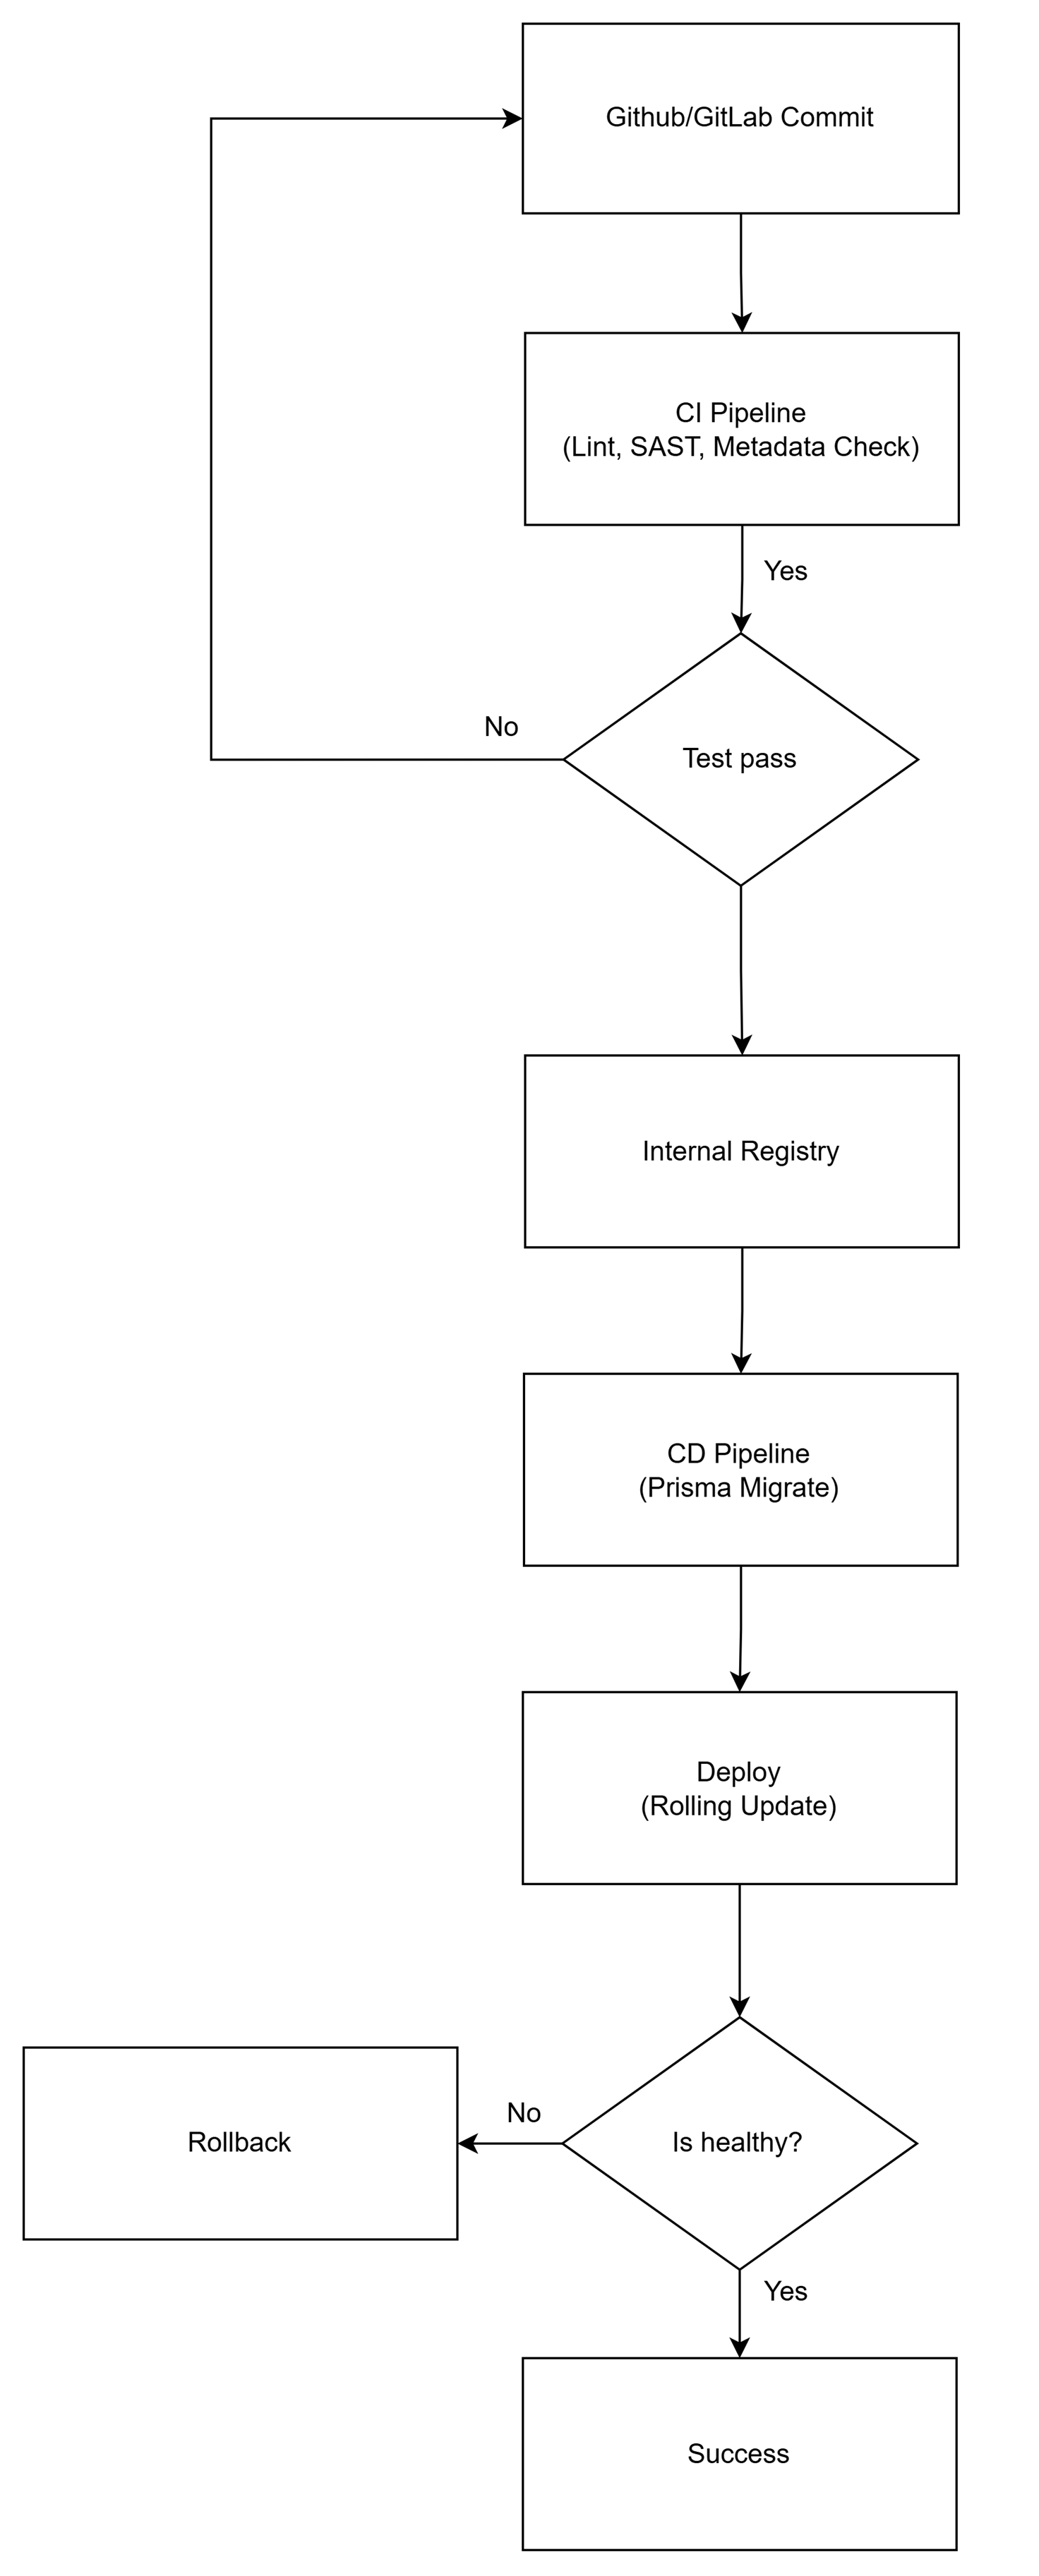
\includegraphics[width=\textwidth, height=0.8\textheight, keepaspectratio]{graphics/cicd.png}
  \caption{Quy trình CI/CD tích hợp kiểm tra dữ liệu và giám sát}
  \label{fig:cicd_process}
\end{figure}

\chapter{Chiến lược Sao lưu và Phục hồi Dữ liệu (Backup Strategy)}
\label{ch:backup_strategy}

Nhóm thực hiện đề xuất giải pháp sao lưu sử dụng \textbf{pgBackRest} kết hợp với hệ thống lưu trữ đối tượng \textbf{MinIO} triển khai nội bộ. Giải pháp này đảm bảo tính bảo mật dữ liệu của trường đại học trong khi vẫn tận dụng được sự linh hoạt của kiến trúc S3.

\begin{table}[H]
\centering
\caption{So sánh MinIO với các giải pháp lưu trữ đám mây}
\label{tab:backup_comparison}
\begin{tabular}{|p{3cm}|p{3.5cm}|p{3cm}|p{3cm}|}
\hline
\textbf{Tiêu chí} & \textbf{MinIO (On-premise)} & \textbf{AWS S3} & \textbf{Google Cloud Storage} \\
\hline
Mô hình triển khai & Private Cloud (Nội bộ) & Public Cloud & Public Cloud \\
\hline
Vị trí dữ liệu & Mạng nội bộ nhà trường & Datacenter nhà cung cấp & Datacenter nhà cung cấp \\
\hline
Khả năng tích hợp & Tương thích hoàn toàn S3 API & Native & SDK riêng \\
\hline
Chi phí vận hành & Thấp (Tận dụng phần cứng sẵn có) & Cao (Theo dung lượng) & Cao (Theo dung lượng) \\
\hline
Độ trễ & Rất thấp (LAN) & Trung bình & Trung bình \\
\hline
\textbf{Độ phù hợp} & \textbf{Rất cao} & Thấp & Thấp \\
\hline
\end{tabular}
\end{table}

\section{Chiến lược và Chu kỳ sao lưu}

Để cân bằng giữa hiệu năng hệ thống và an toàn dữ liệu, hệ thống áp dụng chiến lược sao lưu hỗn hợp:

\begin{itemize}
    \item \textbf{Full Backup (Toàn phần):} Thực hiện \textbf{1 lần/tuần} vào thời điểm thấp điểm (00:00 – 03:00 Chủ nhật). Bản sao lưu này chứa toàn bộ dữ liệu hệ thống.
    \item \textbf{Incremental Backup (Gia tăng):} Thực hiện \textbf{hằng ngày} vào lúc 01:00 sáng. Bản sao lưu này chỉ chứa các dữ liệu thay đổi so với lần backup trước đó, giúp tiết kiệm dung lượng và thời gian.
    \item \textbf{Lưu trữ:} Các bản sao lưu được giữ lại ít nhất 1 tháng (Retention Policy).
\end{itemize}

\section{Phương thức kỹ thuật}

Hệ thống sử dụng công cụ \textbf{pgBackRest} nhờ các ưu điểm vượt trội về hiệu năng và khả năng tích hợp S3. Quy trình xử lý file backup trước khi đẩy lên MinIO bao gồm:
\begin{enumerate}
    \item \textbf{Nén dữ liệu:} Sử dụng thuật toán Gzip/LZ4 để giảm dung lượng đường truyền và lưu trữ.
    \item \textbf{Mã hóa:} Áp dụng mã hóa AES-256 để đảm bảo dữ liệu không thể bị đọc trộm ngay cả khi hệ thống lưu trữ bị xâm nhập.
\end{enumerate}

\section{Cam kết chỉ số phục hồi (RPO \& RTO)}

Dựa trên chiến lược sao lưu toàn phần kết hợp sao lưu gia tăng hằng ngày, hệ thống cam kết:

\begin{itemize}
    \item \textbf{Recovery Point Objective (RPO): 1 ngày.}
    Trong trường hợp xấu nhất, lượng dữ liệu tối đa bị mất tương đương với các giao dịch phát sinh từ sau lần Incremental Backup gần nhất (tối đa 24 giờ).
    
    \item \textbf{Recovery Time Objective (RTO): 1–3 giờ.}
    Thời gian cần thiết để tải các bản backup từ MinIO, giải mã, giải nén và khôi phục vào hệ quản trị cơ sở dữ liệu.
\end{itemize}